\section{Desarrollo}
\subsection{Estructura del proyecto}

Uno de los puntos buenos que tiene este \textit{framework} es
poseer una estructura de directorios bien conocida y definida,
por ello será fácil navegar por ella incluso para nuevos
desarrolladores que se incorporasen al proyecto.

\medskip
Los principales directorios son los siguientes:

\begin{itemize}
    \item /src/app/: ficheros de configuración de la aplicación.
    \item /src/assets/: ficheros multimedia y recursos estáticos.
    \item /src/enviroments/: ficheros de configuración para los
    distintos entornos (desarrollo o producción)
    \item /src/pages/: directorio donde van ubicados los directorios
    de cada pandalla o componente de la aplicación.
    \item /src/pages/page1/: ficheros referentes a una pantalla en
    concreto en el van el HTML, TS, SCSS (si fuese necesario)
    \item /src/providers/: ficheros de acceso a los datos.
    \item /src/theme/: fichero de estilo genérico en el cual
    se basa la aplicación.
\end{itemize}

\medskip
Como se ha indicado anteriormente en el proyecto existen distintos
tipos de ficheros según su objetivo a cumplir, obtener información,
dar formato a los datos para mostrar los mismos, configuración, etc.
A continuación se pasará a mostrar algunos extractos que se han
considerado relevantes.

\begin{figure}
    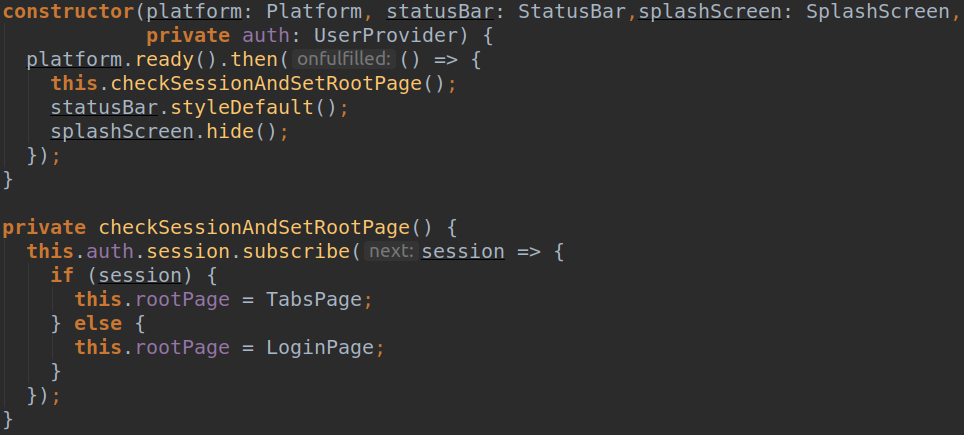
\includegraphics[width=\linewidth]{./images/code/app-components-ts.png}
    \caption{Fichero app.components.ts, control de sesión.}
    \label{app.components.ts}
\end{figure}

\medskip
En la \textbf{figura \ref{app.components.ts}} se puede ver como se gestiona
el control de sesiones. Con ello la aplicación no permite el uso de ninguna
funcionalidad si el usuario no ha iniciado sesión. Como se muestra si el usuario
no ha iniciado la sesión se le enviará a la \textit{LoginPage}. En esta se
permite el inicio de sesión y da acceso al registro para el caso de usuarios
que no se han dado de alta en el sistema. En caso de que si que exista
una sesión por parte del usuario a este se le enviará a la página principal
de la aplicación \textit{TabsPage}. En ella se encuentran las distintas
ventanas disponibles separadas por una barra con pestañas.

\begin{figure}
    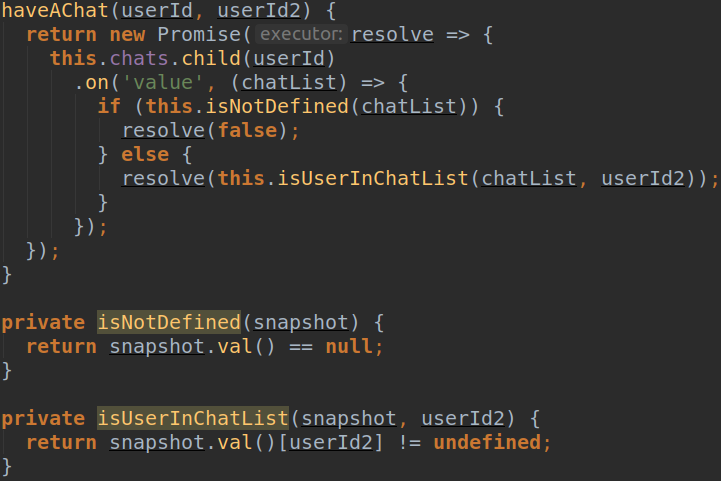
\includegraphics[width=\linewidth]{./images/code/chats-provider-haveAChar.png}
    \caption{Fichero chats.ts, función haveAChat.}
    \label{chats.ts.provider}
\end{figure}

\medskip
En esta \textbf{figura \ref{ejercicios}} se quiere mostrar la importancia que
tienen los nombres en las funciones y la importancia que se le ha dado a
estos durante todo el desarrollo. Se puede ver como con un simple vistazo
cual es el objetivo de esta función, saber si un usuario tiene un
chat abierto con otro. Una vez dentro de esta se puede casi leer como
si de una frase se tratase, "este chat tiene un hijo con este id de usuario
en la lista de chats". Si se continúa leyendo a partir de la línea cinco
se puede leer "si no está definido se resuelve que no tiene un chat y en
caso contrario se comprueba si el usuario está en esta lista y se transmite"

\medskip
Gracias a que se le ha dado buenos nombres a las funciones y parámetros.
Y tratarse de funciones cortas hace que este código sea más legible y entendible sin tener
que realizar grandes esfuerzos. Estas son algunas de las reglas de código limpio \cite{clean-code}
que se han tratado de seguir en este proyecto. Para que el código sea mantenible
de sin tener que utilizar mucho tiempo en comprender lo que se hace en cada parte.
Estas reglas se han considerado
de vital importancia pues se quiere una aplicación longeva que sea fácilmente
sostenible y ampliable, esta tiene que ser en un primer momento, al menos,
entendible por los desarrolladores que se encarguen del mantenimiento de dicho código.


Otra de las leyes o normas que se cumple como consecuencia de usar
buenos nombres, consiste en usar el mínimo posible de comentarios. Al estar bien nombradas
estas funciones, no es necesario añadirles un comentario explicativo sobre la misma.
Es por ello que los comentarios pierden valor.

Por último nombrar un principio más que se puede ver en este
código. Se trata del principio de responsabilidad única, el cual dice
que una función debe cumplir con un único objetivo. Por ejemplo, no debe llamarse
\textit{tieneUnChat} e internamente comprobar si tiene un chat y crear uno en caso de que no lo tenga.
Si fuera así estaría mintiendo con el nombre y se podría hacer un mal uso de esta función.

\begin{figure}
    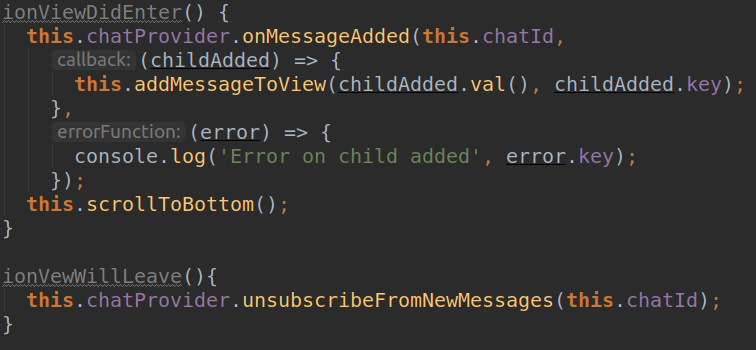
\includegraphics[width=\linewidth]{./images/code/view-chat-ts-onViewDidEnter.png}
    \caption{Fichero view-chat.ts, función onViewDidEnter.}
    \label{view-chat.ts}
\end{figure}

\medskip
Para mejorar la experiencia del usuario se ha tenido en cuenta la carga
de datos. Para ello se ha hecho uso de las funciones que nos da ionic,
como son \textit{ionViewDidEnter} y \textit{ionViewWillLeave}. Las cuales se
ejecutan cuando el usuario abre une nueva ventana y cuando sale de ella, respectivamente.
Es por ello que se realiza la carga de datos por parte del servidor mientras la pantalla se muestra.
De esta manera al no hacerlo en el momento que la pantalla ya está visible por el usuario,
este no tendrá que esperar por los datos en una pantalla en blanco.
Debido a que los datos han sido solicitados al servidor
en el momento que se empieza a preparar la pantalla para mostrarse. De igual
forma este no tendrá que esperar a que se cierre la conexión con la base de
datos para cerrar una pantalla. Dado que en el momento que se comienza la "destrucción"
de la misma el sistema laza la desconexión de manera asíncrona.